\documentclass[tikz,border=1pt,convert=pdf2svg]{standalone}
\usepackage{laser_cut}

\begin{document}
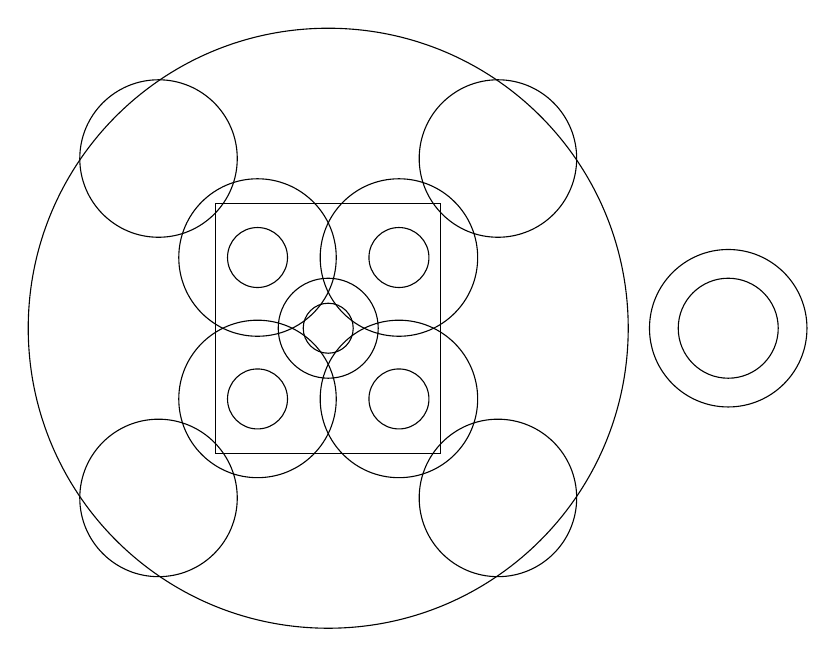
\begin{tikzpicture}
	\node (weight) at (0,0) {};
	\node (washer) at (0,0) {};
	\node (cap) at (2in,0) {};

	\draw (weight) circle (1.5in);
	\foreach \theta in {45,135,...,315} {
		\draw (weight)++(\theta:1.2in) circle (\sixthirtytworadius);

		% standoffs
		\draw (weight)++(\theta:0.5in) circle (\sixthirtytworadius);
		\draw (weight)++(\theta:0.5in) circle (0.15in);
	}
	\node[draw,shape=rectangle,minimum width=1.125in,minimum height=1.25in,anchor=center] at (weight) {};

	\draw (washer) circle (0.25in/2);
	\draw (washer) circle (0.5in/2);

	\draw (cap) circle (\sixthirtytworadius);
	\draw (cap) circle (0.5in/2);

\end{tikzpicture}
\end{document}


